\documentclass{beamer}

\usepackage{slashed}
\usepackage{braket}
\usepackage{subcaption}
\usepackage{bm}
\renewcommand\vec\bm

\usetheme[block=fill]{metropolis}

\author{Thorvald M. Ballestad}
\title{Master thesis presentation}
\date{03. June 2022}
\titlegraphic{
  \vspace{5cm}
  \flushright
  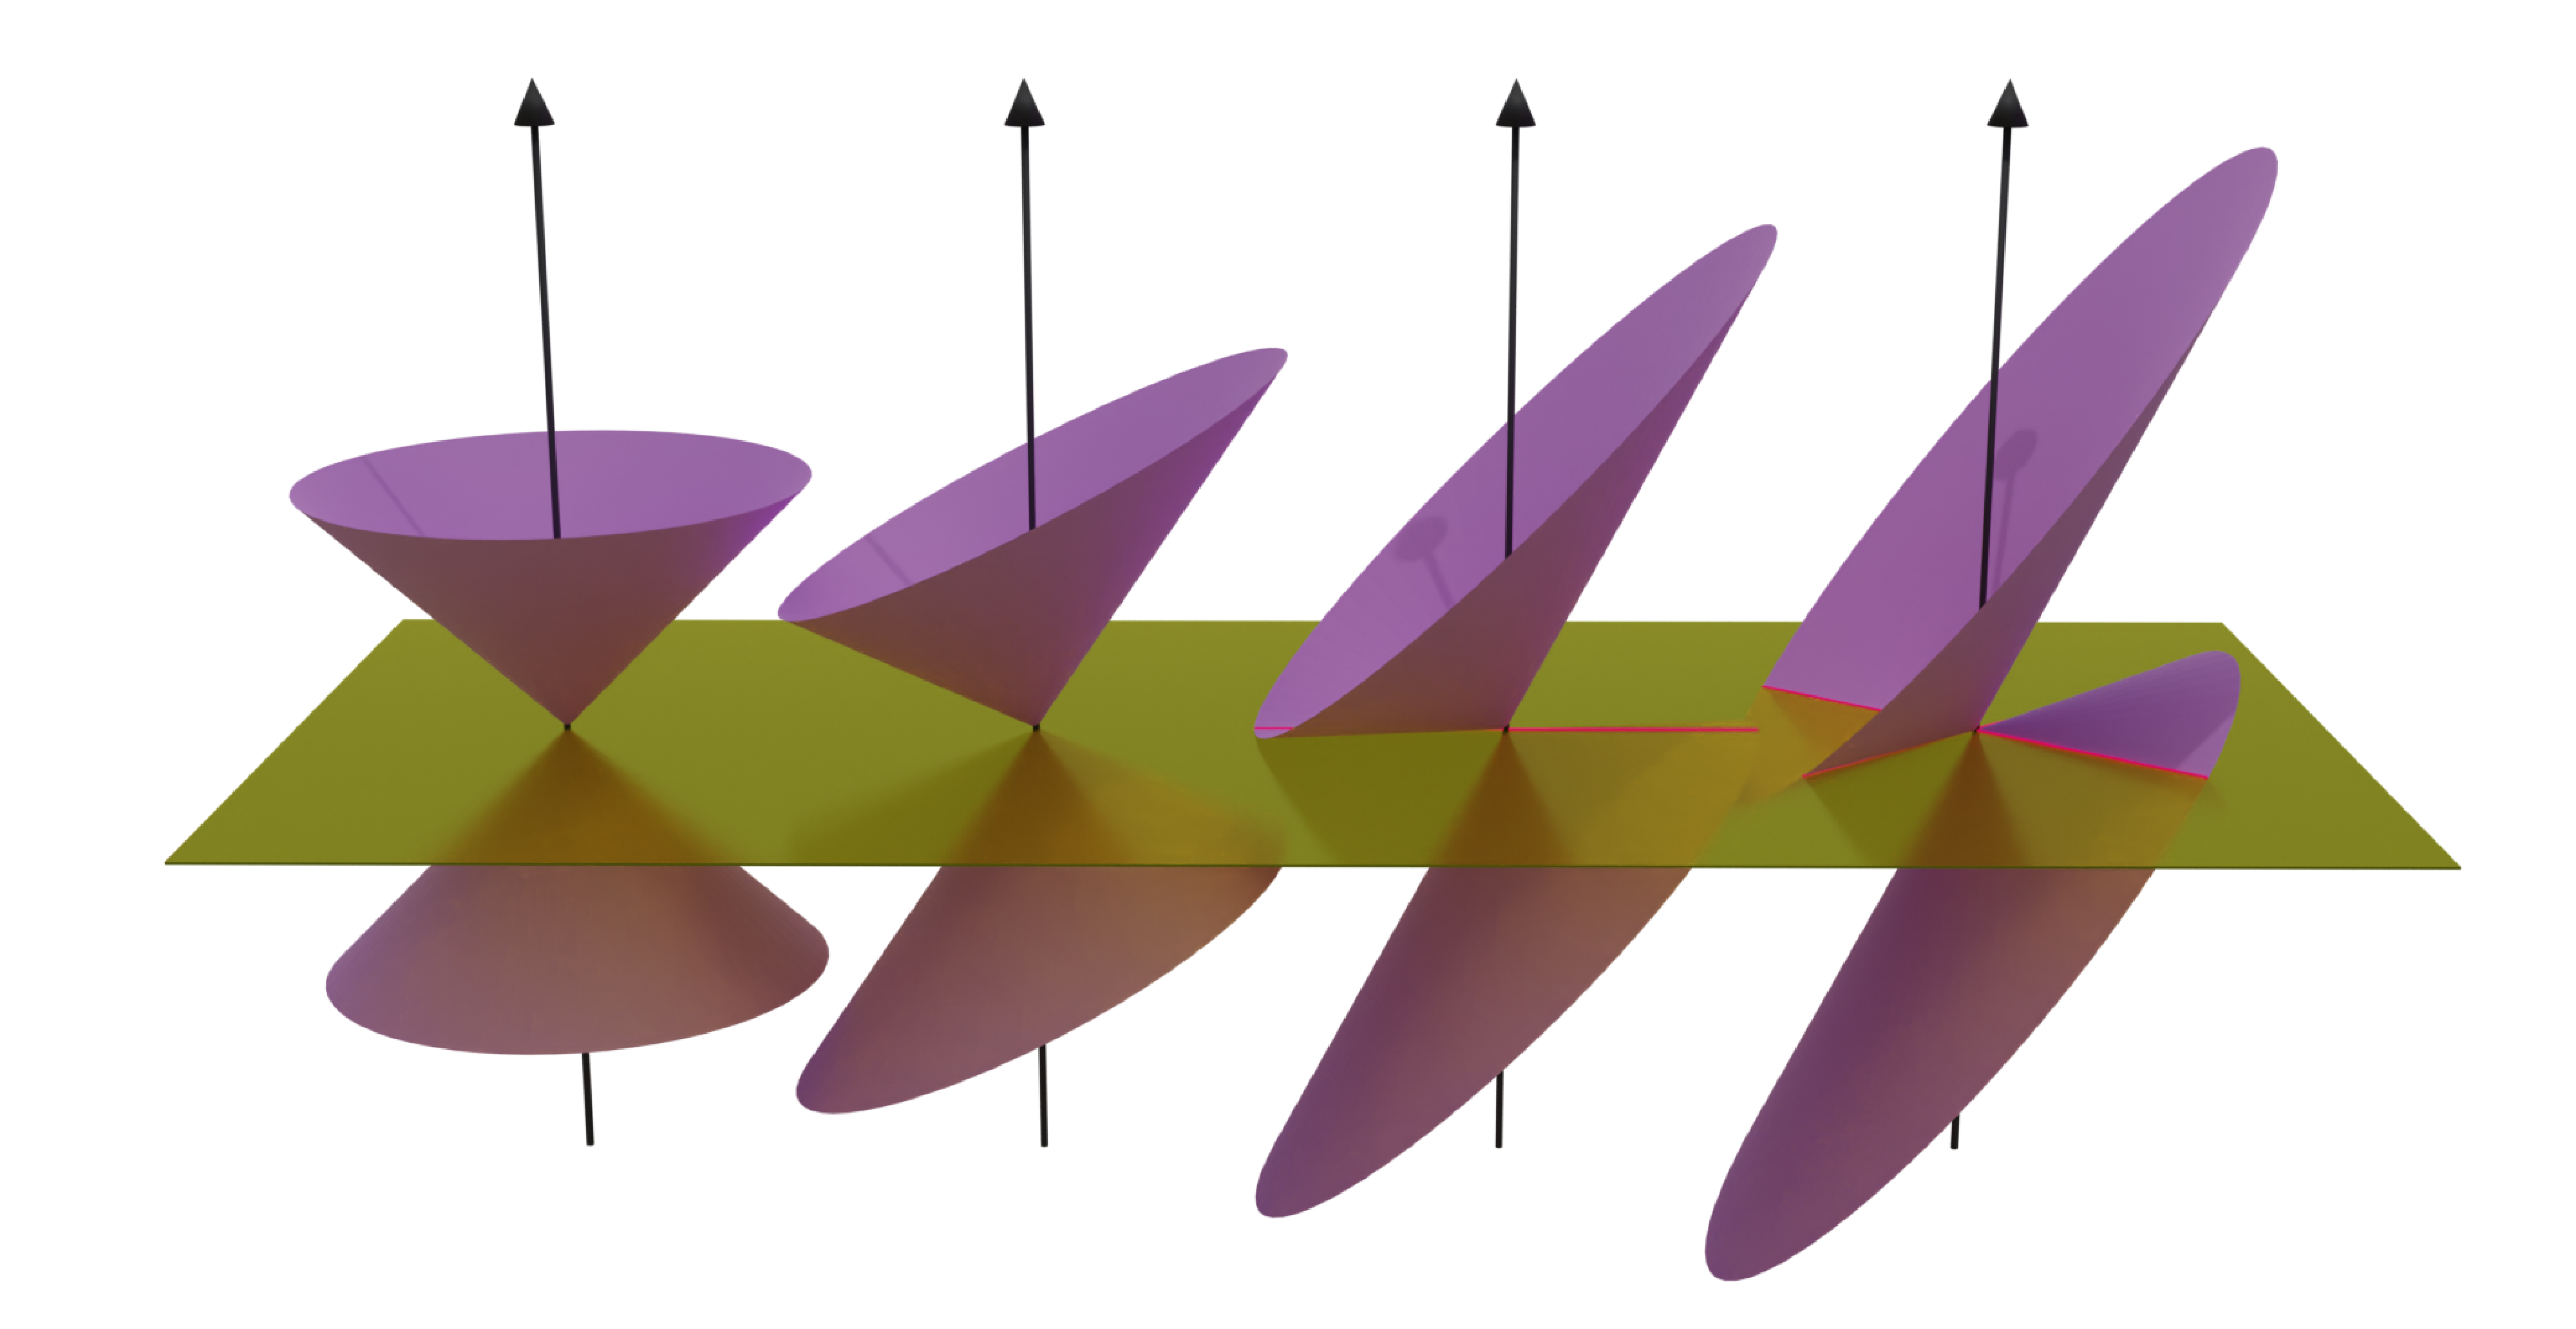
\includegraphics[width=.6\textwidth]{cones-tilt-color1}
}

\begin{document}
\begin{frame}
\titlepage
\end{frame}

\section{Background}
\begin{frame}{Conformal anomaly in massless QED}
  The massless Dirac equation
  \begin{equation}
    \label{eq:1}
    \bar{\psi} i \slashed{\partial} \psi = 0.
  \end{equation}
  Conformal anomaly in small perturbation limit
  \begin{equation}
    \label{eq:5}
    g^{\mu \nu} = \eta^{\mu \nu} + \delta g^{\mu \nu}.
  \end{equation}
  The Dirac cone Hamiltonian
  \begin{equation}
    \label{eq:2}
    H_D = v_F s \vec{p} \vec{\sigma}.
  \end{equation}
  % \begin{center}
  %   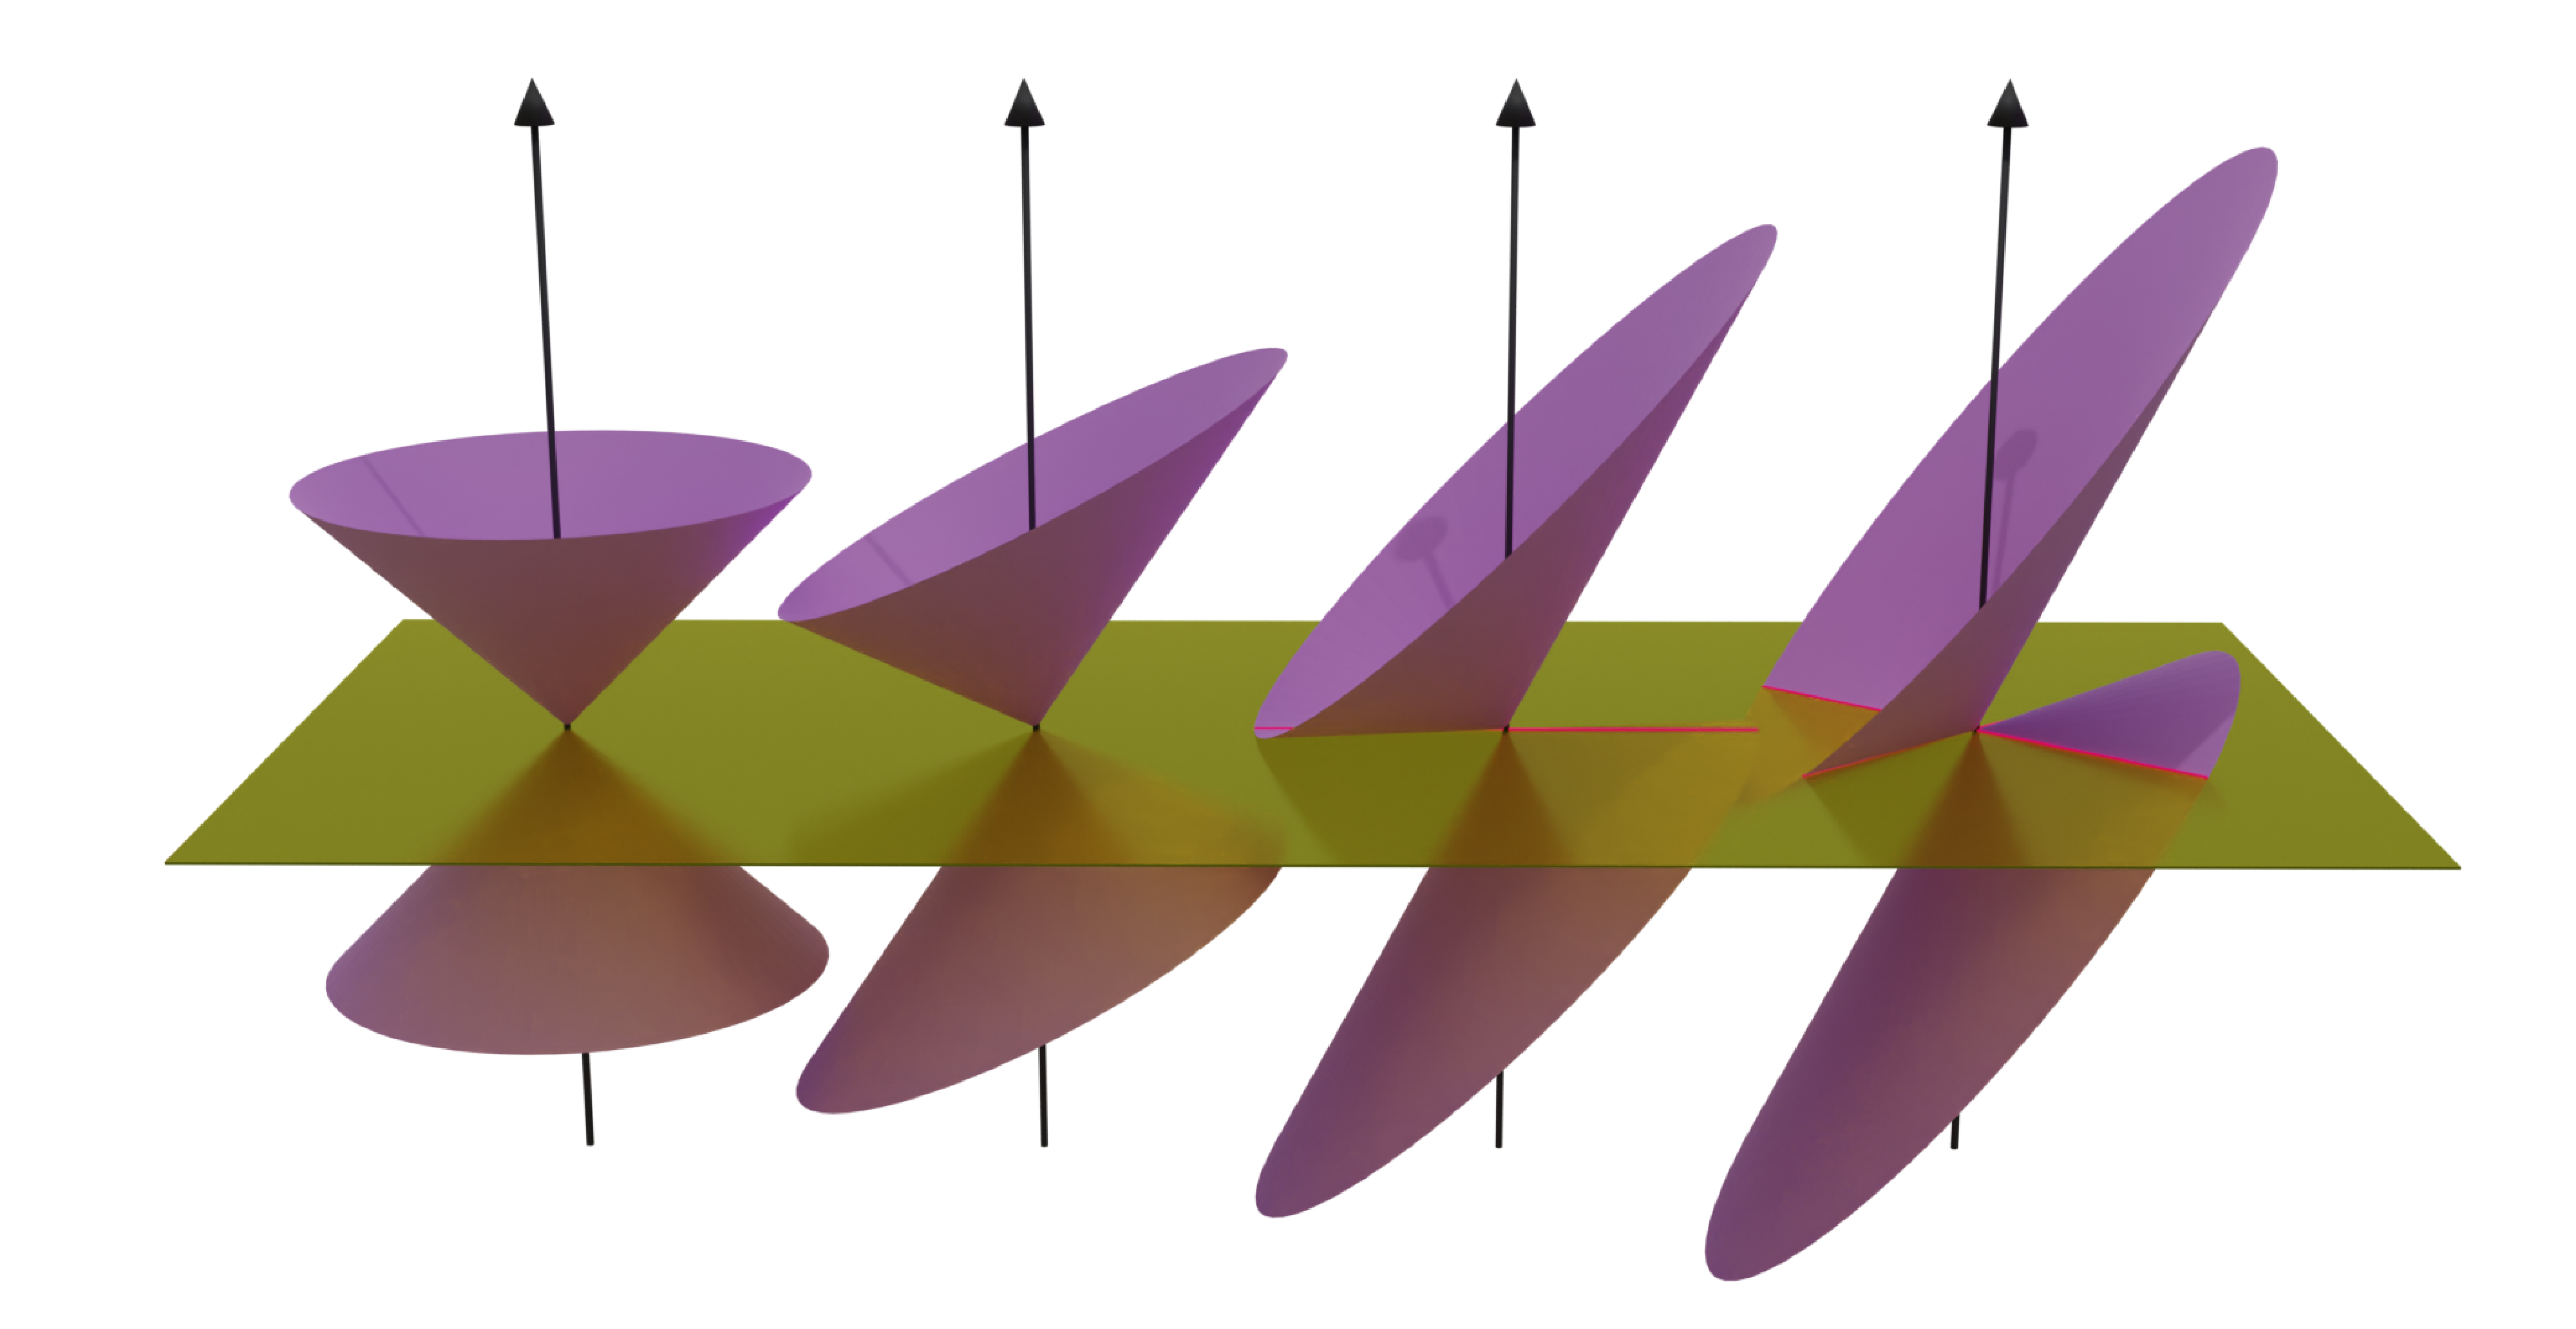
\includegraphics[width=0.6\textwidth]{cones-tilt-color1}
  % \end{center}
\end{frame}

\section{Our work}
\begin{frame}{Linear response and Luttinger's method}
  Temperature pertupation \( \nabla T \) and gravitational potential \( \psi \)
  \begin{equation}
    \label{eq:3}
    \nabla \psi + \frac{\nabla T}{T} = 0.
  \end{equation}

  Linear response (Kubo)
  \begin{multline}
    \label{eq:4}
    \Braket{J^{}}(t, \vec{r}) =
    iv_F
    \int \mathrm{d}t' \mathrm{d} \vec{r}'
    \int_{-\infty}^{t'} \hspace{-1em} \mathrm{d}t''
    \Theta(t-t')\\
    \times
    \Braket{\left[
      \vec{J}^i(t, \vec{r})), T^{j0}(t'', \vec{r}')
\right      ]}
\frac{\partial_j' T(t', \vec{r}')}{T(t', \vec{r}'}
  \end{multline}
\end{frame}
\begin{frame}{Type-I and Type-II}
  \centering
  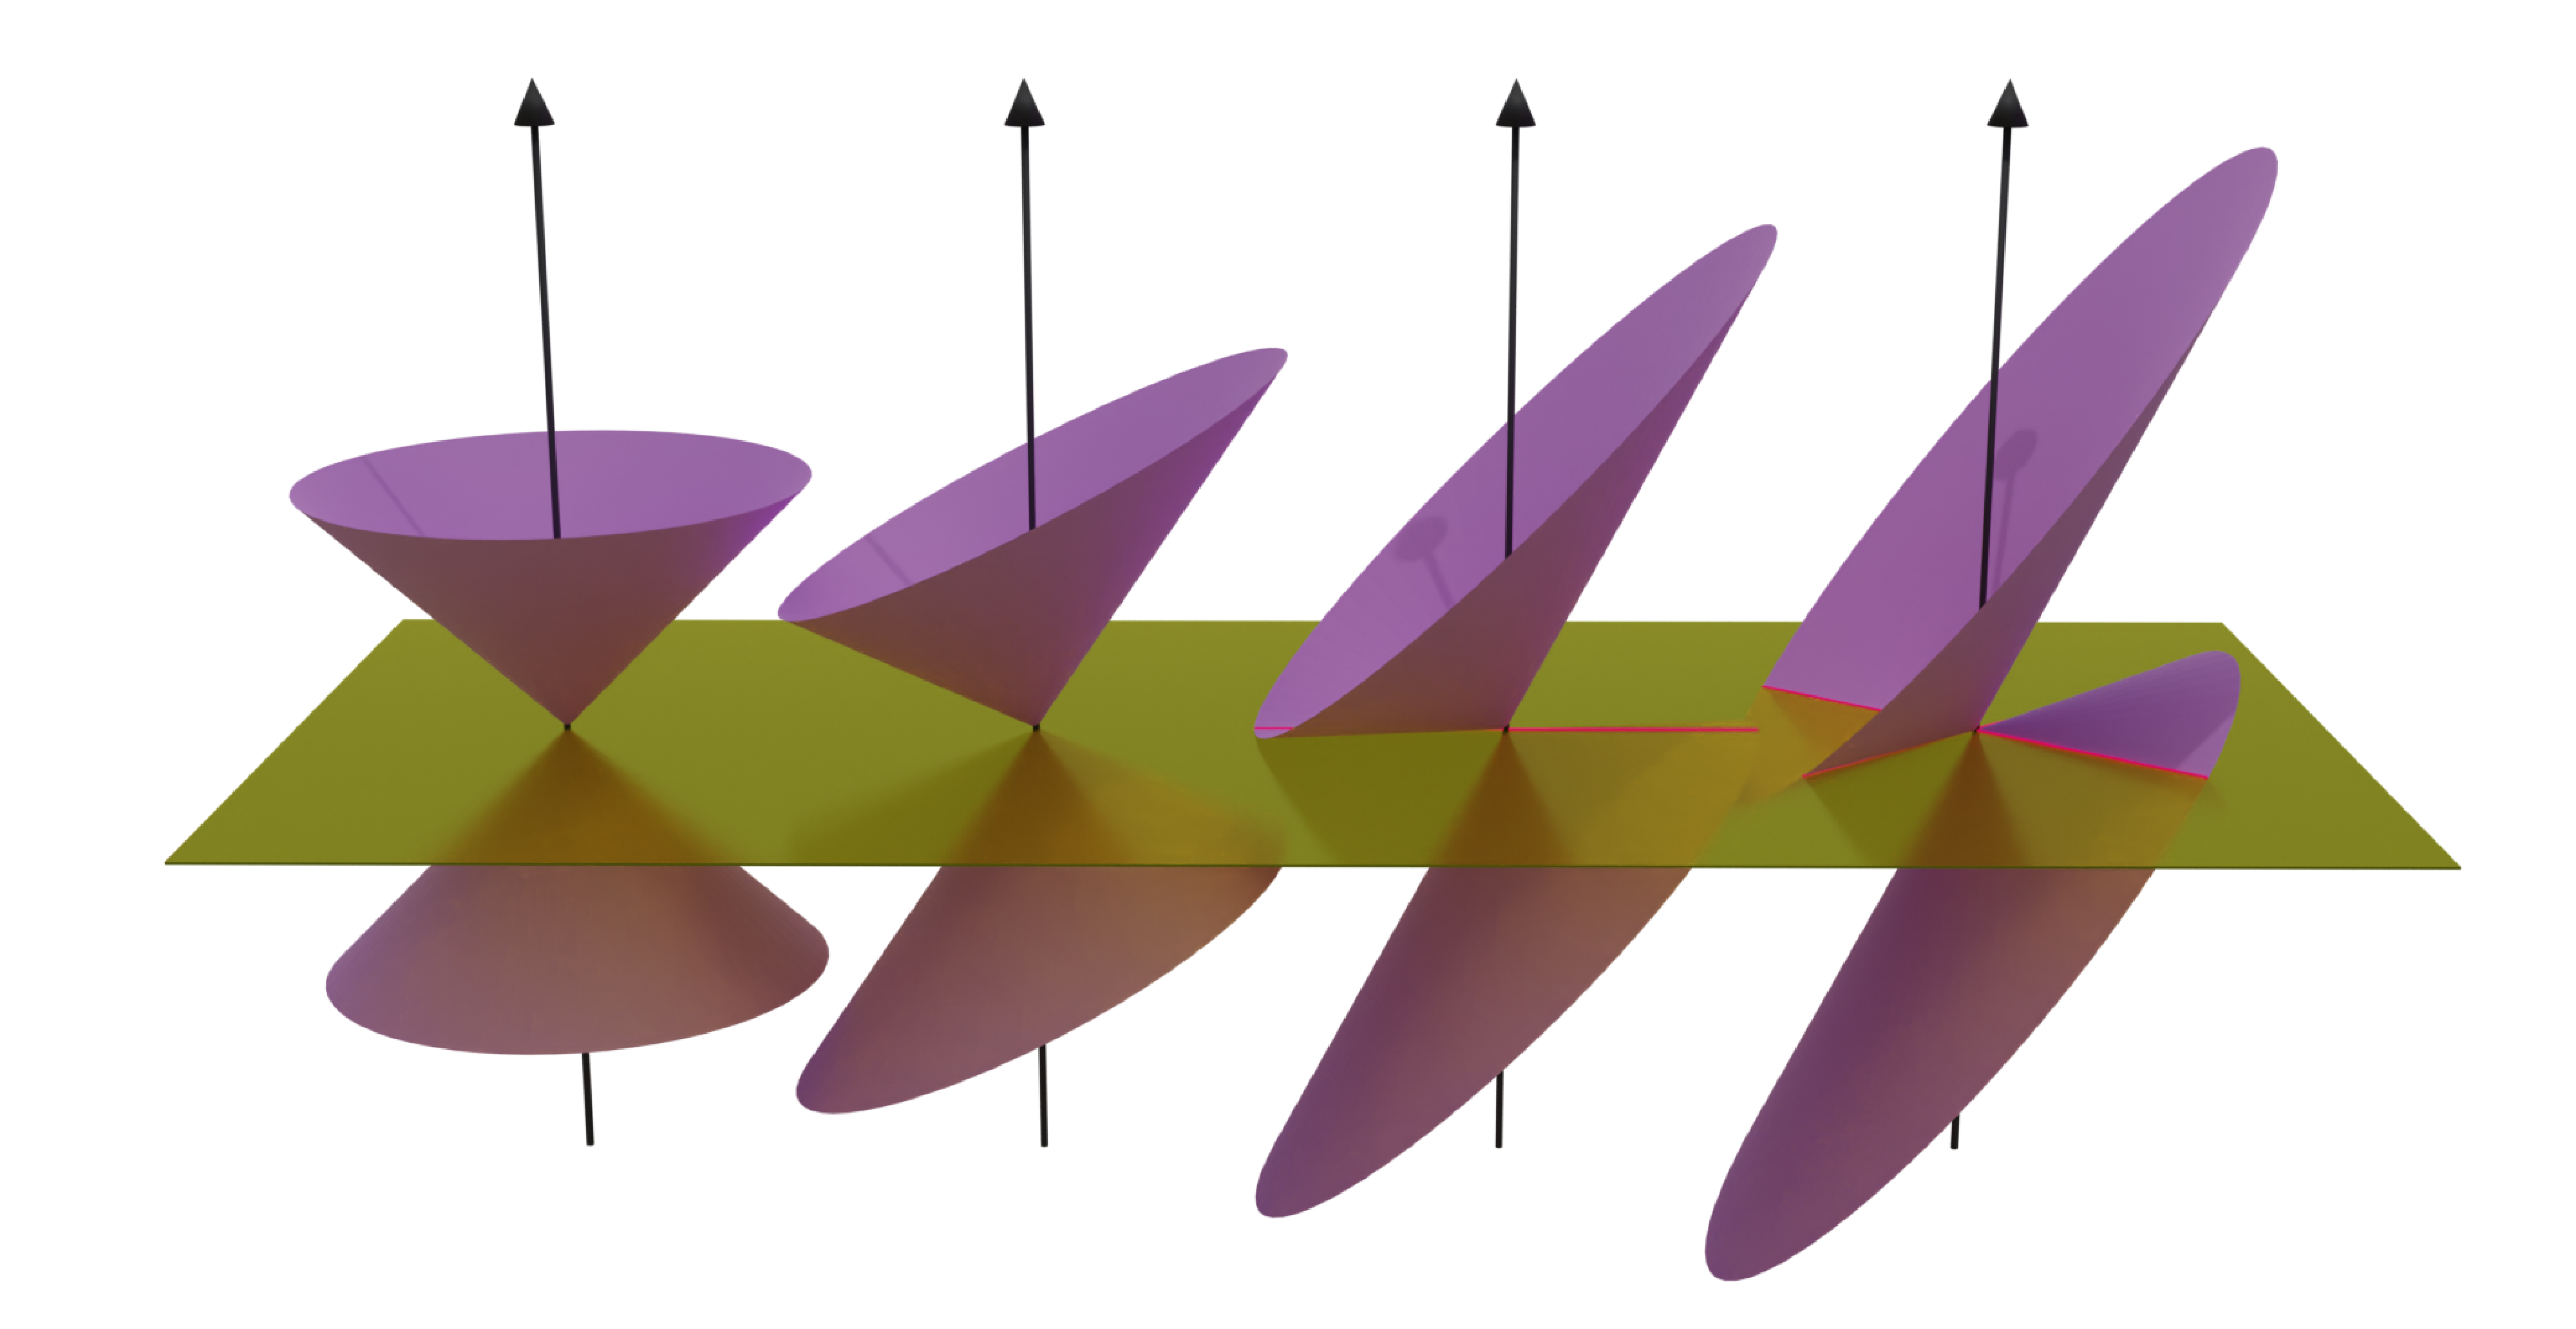
\includegraphics[width=.7\textwidth]{cones-tilt-color1}
\end{frame}
\begin{frame}{Landau levels}
  \begin{center}
    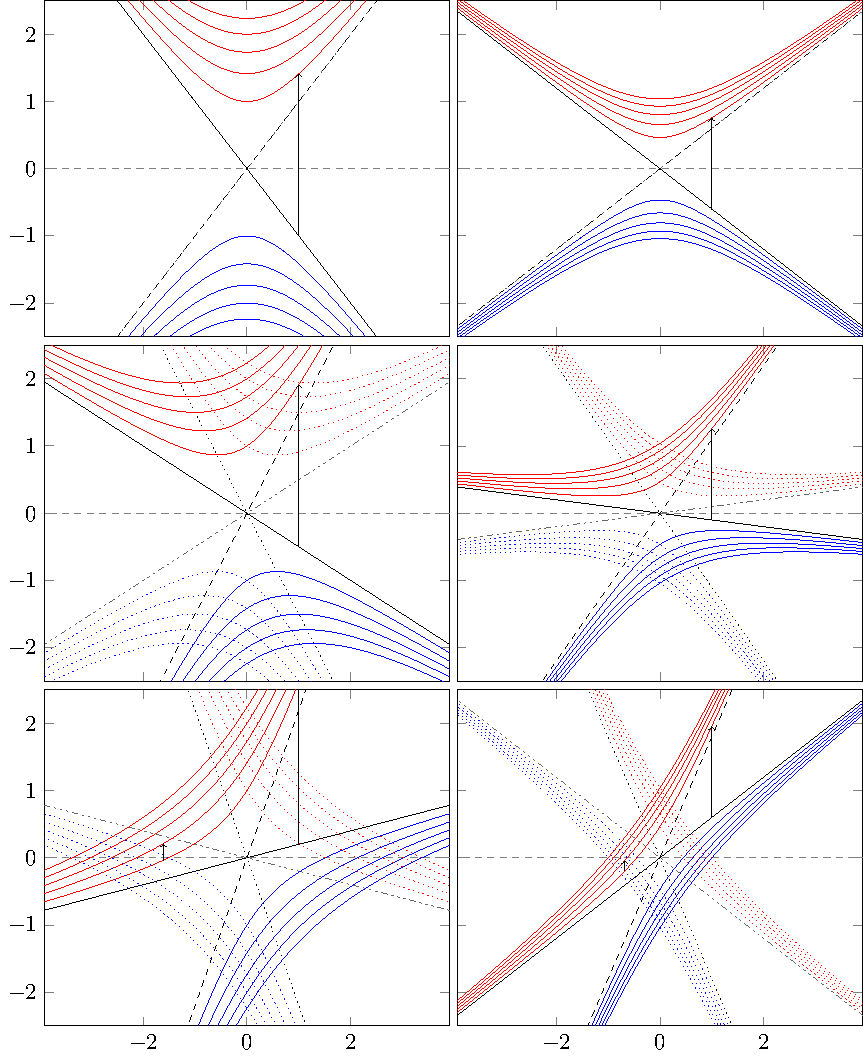
\includegraphics[width=0.4\textwidth]{lllevels}
  \end{center}
\end{frame}
\begin{frame}{Type-I and Type-II}
  \centering
  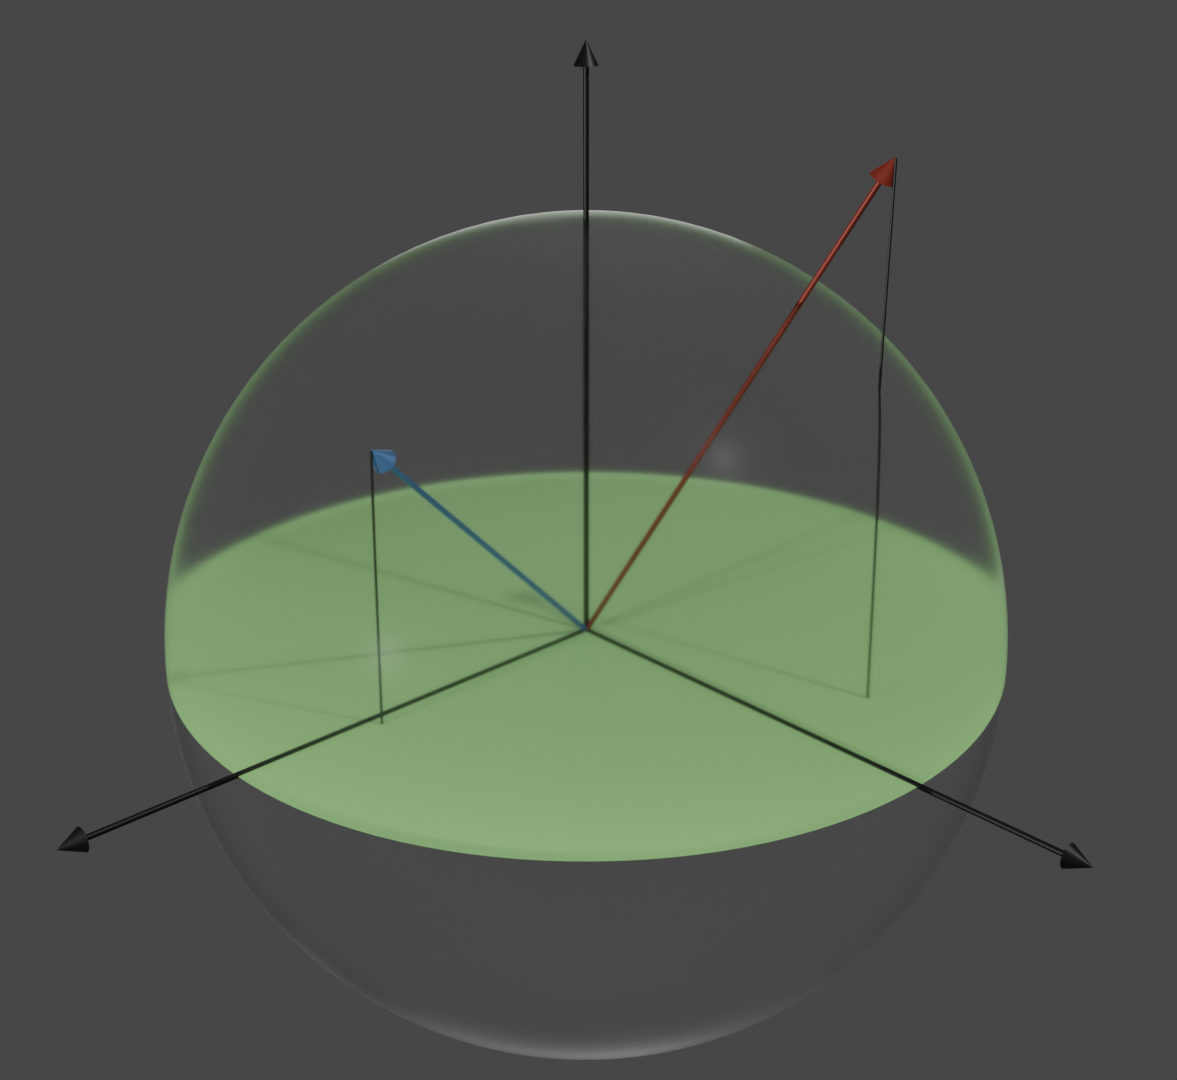
\includegraphics[width=.5\textwidth]{tiltSpherewBackground}
  \begin{block}{Proposition}
    The modulus of the \emph{tilt vector} \( \vec{t} \) separates Type-I from Type-II, with Type-II having \( t > 1 \).

    Collapse of LLs for perpendicular tilt.
  \end{block}
\end{frame}
\begin{frame}[standout]
  \metroset{background=dark}
  \begin{block}{Result}
    The response can be directly tuned by the \emph{tilt parameter} \( \vec{t} \).
  \end{block}
\end{frame}
\begin{frame}{Perpendicular tilt}
  \centering
  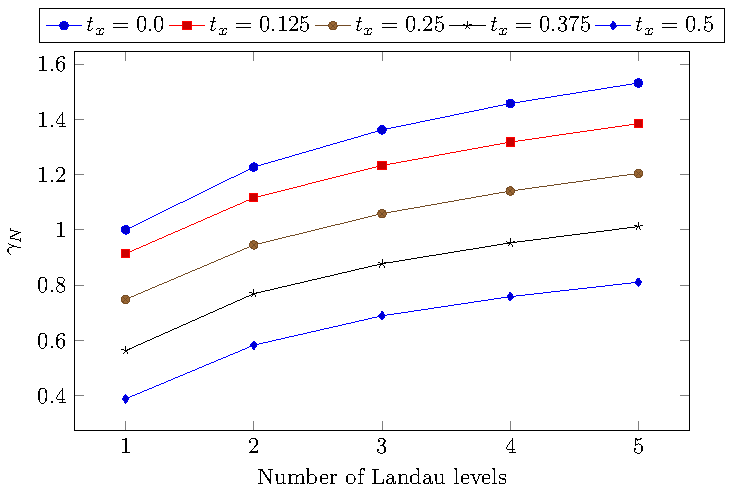
\includegraphics[width=.7\textwidth]{contribtx}
\end{frame}
\begin{frame}{Parallel tilt}
  \begin{figure}
    \subcaptionbox{Type-I}{
      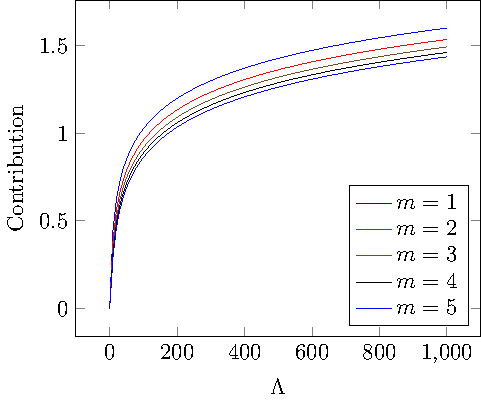
\includegraphics[width=.3\textwidth]{divergentContribCutoff}
    }
    \subcaptionbox{Type-II inter band}{
      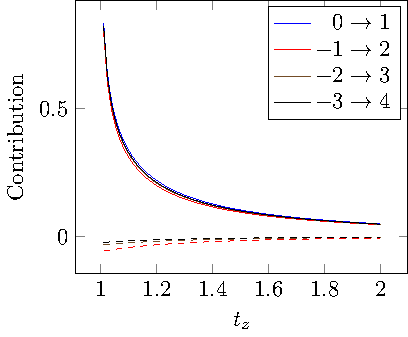
\includegraphics[width=.3\textwidth]{tzcontribtypeii}
    }
    \subcaptionbox{Type-II intraband}{
      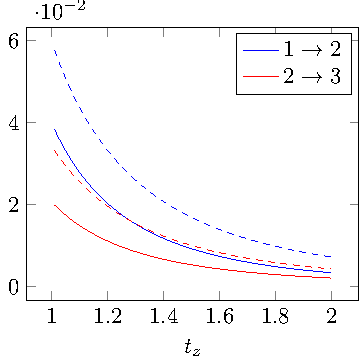
\includegraphics[width=.3\textwidth]{tzcontribtypeii_intraband}
    }
  \end{figure}
\end{frame}
\begin{frame}[standout]
  \metroset{block=transparent}
  \begin{block}{}
    \centering\Huge
    Thank you!
  \end{block}
\end{frame}

\appendix
\begin{frame}

\end{frame}
\end{document}
